\section{Experiments}
\label{exp}
In this section we will briefly explain our robotic platform, experimental setup and the set of experiments along with the metrics which have been conducted to evaluate the performance of our system.

\subsection{Robotic Platform}
\label{sec:robot}

\begin{figure}[t!]
\centering
\subfloat[]{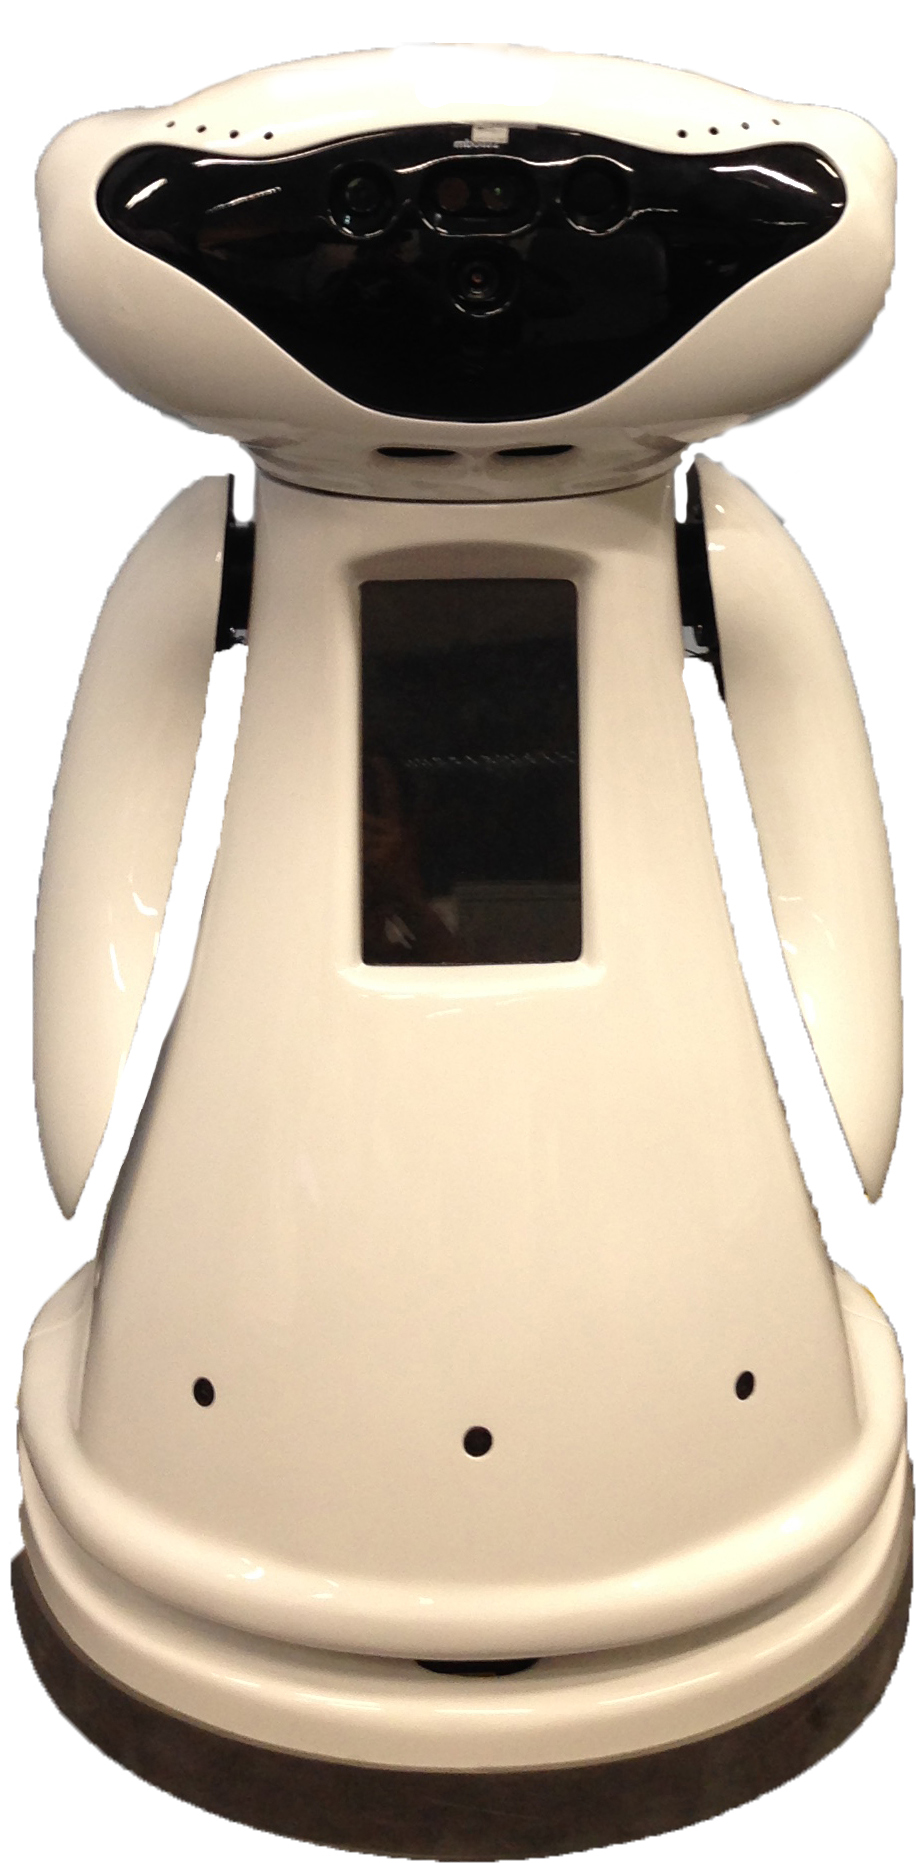
\includegraphics[width=0.13\textwidth]{pictures/robot.jpg}\label{fig:robot}}%
\hspace{0.4cm}
\subfloat[]{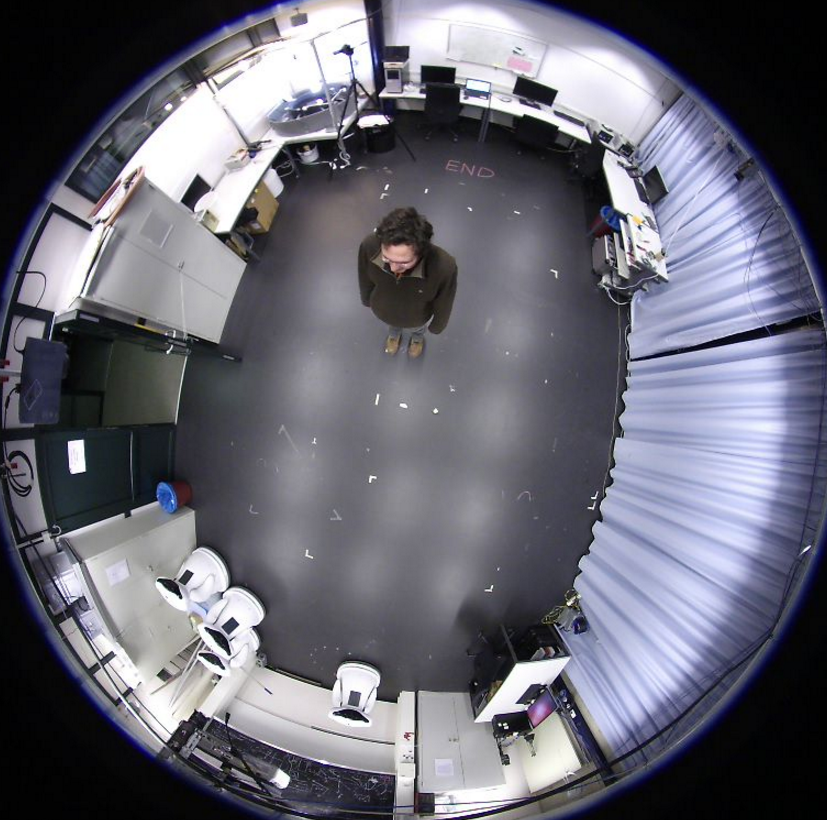
\includegraphics[width=0.3\textwidth]{pictures/arena.png}\label{fig:arena}}%
\hspace{0.1cm}

\caption{(a) mBot robotic platform. (b) Experimental arena. The robot starts from its initial position and navigates to the end point while dealing with the people in the environment. This is a snapshot of the first step of the single static person case.}
\label{fig:setup}
\end{figure}


%\begin{figure}
%    \centering
%    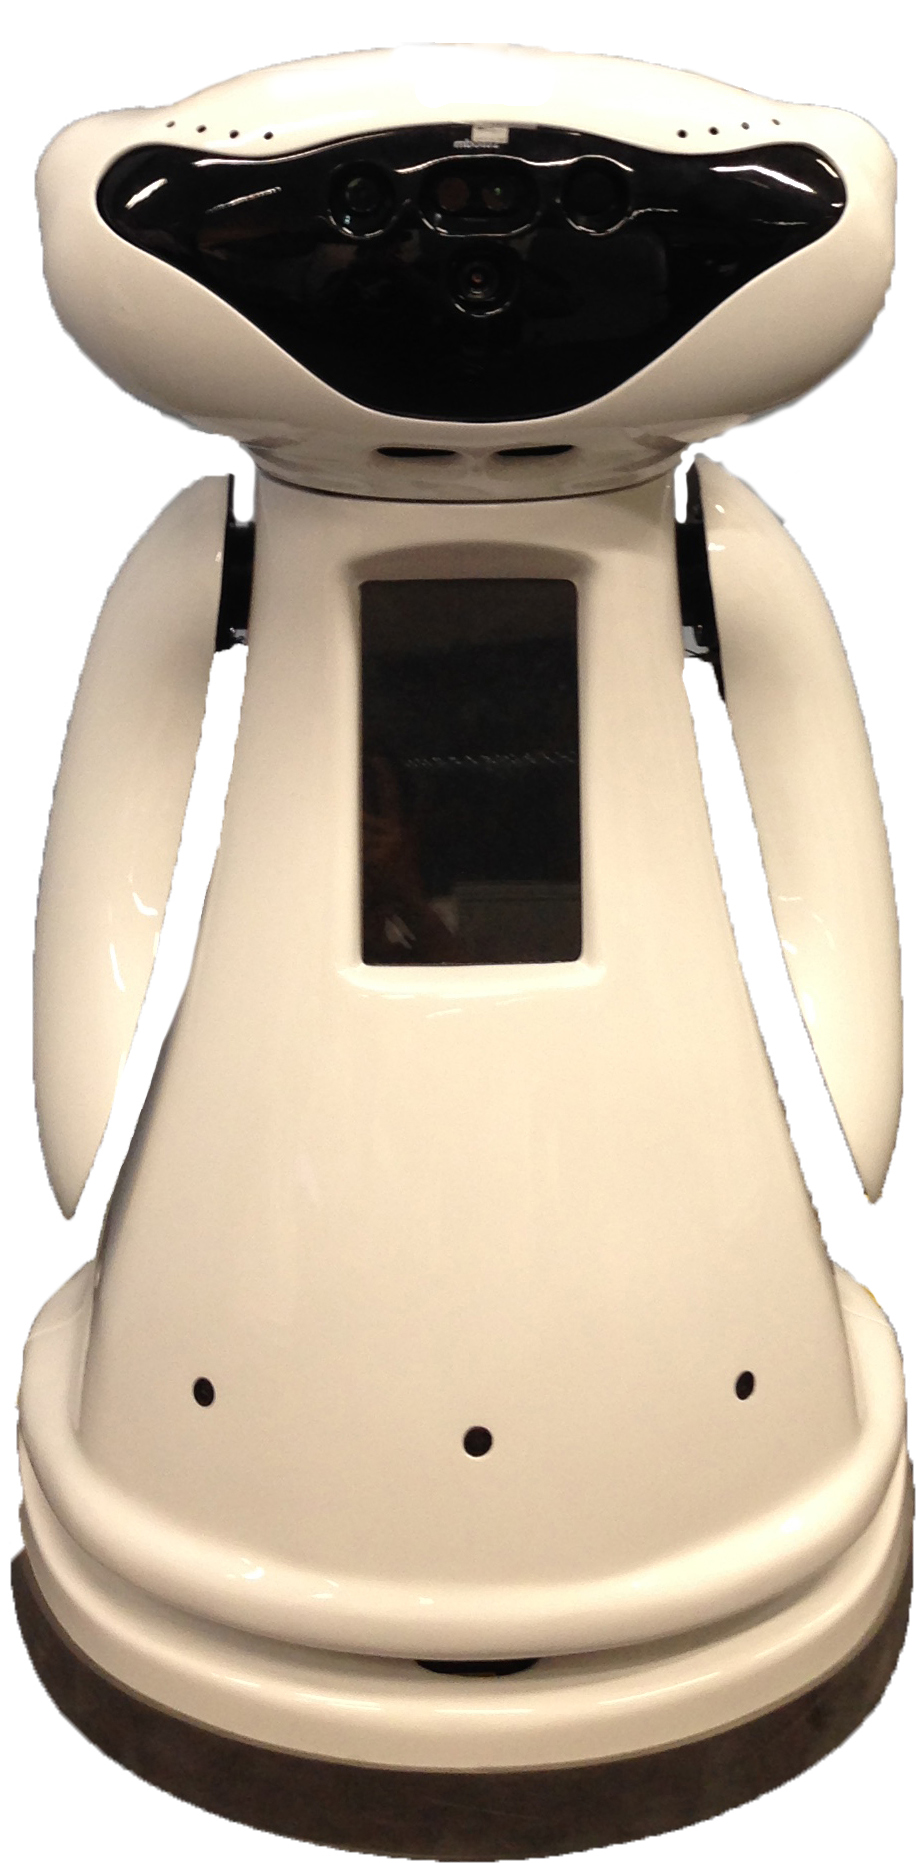
\includegraphics[scale=0.07]{pictures/robot.jpg}
%    \caption{Robot used in our experiments to perform the automatic fingerprinting.}
%     \label{robot}
%\end{figure}


The robotic platform used in this work is shown in Fig. \ref{fig:robot}. This robot is called mBot \cite{Messias2014robotic} and is developed within the FP7 European project MOnarCH.
It is an omni-directional drive robot with an approximately round footprint of 0.65~\textit{m} in diameter and a height of 0.98~\textit{m}.
It is provided with two laser range finders, on both the front and the back for providing full coverage.

Two batteries give it an autonomy of approximately five hours, depending on the usage.
The robot has two PCs inside its shell: one manages the sensors, navigation and actuators, while the second one is for other functions such as human-robot interaction functionalities, which are outside our interests for this work. The two on-board PCs, run Ubuntu desktop 12.04 and ROS Hydro. 


\subsection{Experimental Setup}
\label{sec:Experimental_setup}


We have used an extensive suit of experiments both in simulation and reality, for performance evaluation. A high fidelity robotic simulator Webots \cite{michel1998webots}, with realistic models of the mBot and the testing environment has been used for evaluations in the initial step. The trackers have been emulated initially, but real recorded data bags of perception were used in the next steps for more close to reality simulations. This was done to simplify the debugging process and speeding up the robotic experiments. %by replaying real uncertainty and tracking data from real experiments.
Finally, we tested our methods in reality in three different scenarios, in a laboratory environment of 5~\textit{m}~$\times$~7~\textit{m}, depicted in Fig. \ref{fig:arena} where the tracker was operational.
 
%\begin{figure*}[t]
%\centering
%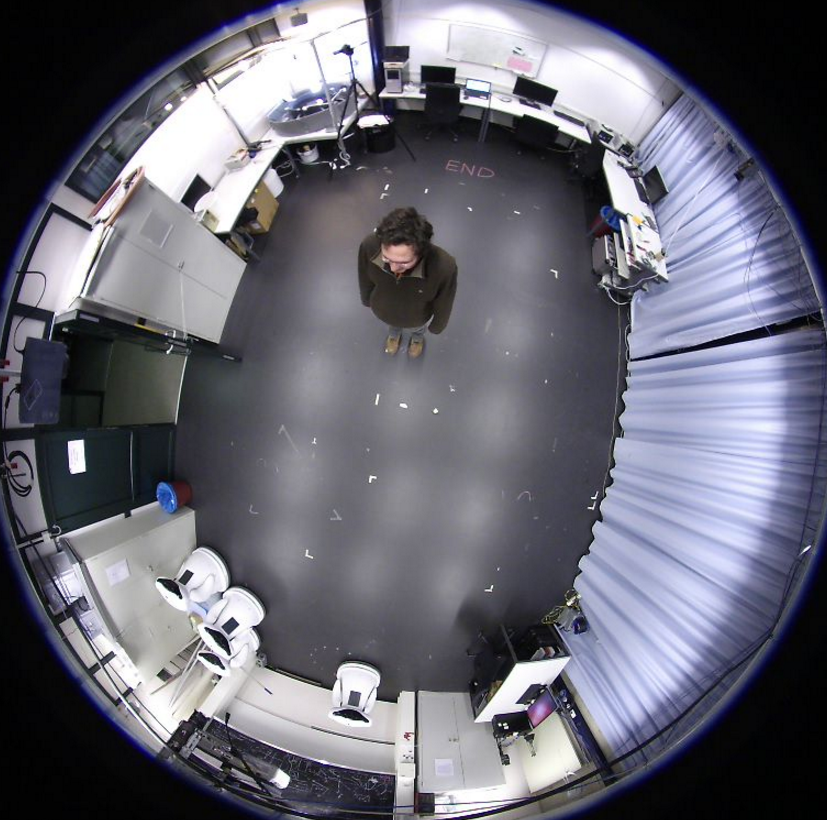
\includegraphics[width=0.30\textwidth]{pictures/arena.png}
%\caption{Connection of different system components.} %The social navigation layer adds the costs associated to people to other costmaps for taking path planning decisions.}
%\label{fig:arena}
%\end{figure*}


People detection and tracking is done by means of a networked omni-directional cmaera with 180 degrees field of view. The tracker outputs results at the rate of 3~\textit{Hz}. The ground truth position of the robot is given by AMCL with 5-10~\textit{cm} accuracy, and the person stands and walks on physically marked tracks to get the exact precise ground truth.
The control rate of navigation is 20~$Hz$ while the social costmap generation has a rate of approximately 3~\textit{Hz}. This is to account for the low output frequency of the tracker.


\subsection{Scenarios}
\label{sec:scenarios}

We have studied three different scenarios, each having been tested five times. We start with 1) a single static person and incrementally increase the complexity to 2) one moving person and finally, 3) two static people in the arena. it should be emphasized that perception uncertainty is affecting the tracking performance and is not evident or quantifiable from just looking at the environment. This means, the person is not aware of what is happening on the tracker side, however, the information given by the tracker greatly affects the behavior of the robot, and therefore the social acceptability. 


Since we aim to study the effect of perception uncertainty in human-aware navigation, we chose a task of point to point navigation for the robot in the vicinity of humans, which is the most general and basic navigation task. The complexity of the navigation task can be increased and more interesting scenarios in terms of Human Robot Interaction (HRI) can be investigated, but that is outside the scope of this work. 

In each experiment, the robot starts from a predefined starting point and is sent to one predefined goal. The robot then has to behave appropriately when encountered with people in the arena. For the static case there is always a person standing between the robot and the straight line to the goal, and for the dynamic case the person moves along this line in the opposite direction, as the robot starts navigating towards the goal, causing a direct encounter with the robot. The following section will explain the metrics used for performance assessment.% in our experiments.

%
%Figure shows a snapshot of the setup with two people moving in the arena. For the case of static people we have also done extensive tests using a high fidelity simulator webots \cite{michel1998webots}, by 1) emulating the uncertainty of tracking, and 2) replaying real uncertainty and tracking data from real experiments. 




\subsection{Metrics}

Six different metrics have been defined for performance evaluation. A subset of these metrics is chosen for each experiment based on the scenario of interest.% Table \ref{table:metrics} briefly describes each of the metrics and the scenarios they have been used for.


\begin{itemize}

\item $m_{1}$: Shows the minimum distance that the robot has kept during the experiment to a human. If this distance is not large enough, the robot will be invading the personal space of the person and will therefore cause discomfort. 


\item $m_{2}$: Shows how long the robot has been moving in areas associated with social costs. This means, whenever the robot is in a position with corresponding non-zero value in the costmap this metric will be incremented.

 \item $m_{3}$: Shows the accumulated social cost, this is to differentiate between being in different positions of the social costmap, which is not reflected in $m_{2}$.
 So if the robot is closer to a person, the social cost will be higher and this metric will increase. For more information on $m_{1}-m_{3}$ refer to \cite{talebpour2015board}. 

\item  $m_{4}$: Shows the smoothness of the robot trajectory. This is important from the human observer's point of view when perceiving the robot motion. Humans are known to prefer motion with minimum jerk \cite{sisbot2010synthesizing}, therefore we took the root mean squared error (RMSE) of the trajectory jerk in $m_{4}$:
\begin{equation}
r_{t} = \begin{bmatrix}
x_{t}\\
y_{t} 

\end{bmatrix} \, , \, \,  m_{4} = \sqrt{\frac{1}{N} \sum_{t=1}^{N}\left | \dddot{r_{t}} \right |^{2}  }
\end{equation}
$r_{t}$ indicates the position of the robot at time $t$, and $N$ indicates the total time of the experiment. It should be emphasized that we did not actively try to modify the robot control to get smoother trajectories, we are just interested to see which method results in a more natural and smooth path.  

\item $m_{5}$: Is the total time steps required to finish the navigation task.


\item $m_{6}$: Shows the minimum average distance to the people present in the environment. This is interesting since it shows how the robot is choosing to use the space. Does it choose to go through the area between the people or does it prefer to take a tour and increase this minimum average distance.

\end{itemize}

%\begin{table}[h!]
%\centering
%\begin{tabular}{||c l c||} 
 %\hline
 %Name & Description & Scenario \\ [0.5ex] 
 %\hline\hline
 %$m_{1}$ & Minimum distance to a person (\textit{m}) & 1,3 \\ 
 %$m_{2}$ & Time steps spent in areas with social cost & 1,3  \\
 %$m_{3}$ & Accumulated social cost & 1,3  \\
 %$m_{4}$ & Smoothness of the trajectory & 1,2,3  \\
% $m_{5}$ & Time steps to finish the task & 1,2,3  \\
 %$m_{6}$ & Minimum average distance to the people (\textit{m}) & 3  \\ [1ex] 
% \hline
%\end{tabular}
%\caption{Performance metrics.}
%\label{table:metrics}
%\end{table}


